\documentclass[11pt]{amsart}
\usepackage[a4paper,margin=1in]{geometry}
\usepackage{amssymb}
\usepackage{graphicx}
\usepackage{tikz}
\usepackage[hidelinks]{hyperref}
\hypersetup{pdftitle={Random Chords of Two Circles and a Third Centre},pdfauthor={Vamshi Jandhyala}}

\newtheorem{theorem}{Theorem}
\newtheorem{lemma}[theorem]{Lemma}
\newtheorem{corollary}[theorem]{Corollary}
\theoremstyle{remark}
\newtheorem*{remark}{Remark}

\newcommand{\R}{\mathbb{R}}
\newcommand{\E}{\mathbb{E}}
\newcommand{\eqd}{\overset{d}{=}}

\title[Random Chords of Two Circles]{Random Chords of Two Circles and a Third Centre}
\author{Vamshi Jandhyala}
\date{Preprint, version 1, 8 October 2026. Not peer reviewed.}
\subjclass[2020]{Primary 60D05; Secondary 52A22}
\keywords{geometric probability, random lines, arcsine law, tangent circles}

\begin{document}

\begin{abstract}
Choose independent uniform points $A$ and $B$ on two circles whose discs have disjoint interiors. We show that the angles between the normal of the line $AB$ and the radii to $A$ and to $B$ are independent and uniform. Equivalently, the signed offsets of the line from the two centres, each divided by its radius, are independent with the arcsine law. From this we characterise when a point $O$ on the line of centres sees the line $AB$, and the chord $BC$ through a second uniform point $C$ of the second circle, at the same distance in distribution: exactly when $O$ is the second centre, or when the circles touch and $O$ lies beyond the second circle at a distance from its centre equal to $b(a+b)/a$, where $a$ and $b$ are the radii. This answers a question of Dan on MathOverflow about three touching circles with radii in geometric progression, extends it to every circle about the third centre and to chains of circles, shows that the progression is necessary for equality of the distance distributions, and gives a single elementary integral for the common hit probability at every radius ratio.
\end{abstract}

\maketitle

\noindent\emph{Status of this preprint.} This version has not yet been independently reviewed.

\section{A question to try}

Three circles touch in a row with collinear centres $P$, $Q$, $O$ and radii $a$, $b$, $c$. Choose $A$ uniformly on the first circle and $B$, $C$ uniformly on the second, all independent, and draw the lines $AB$ and $BC$ (Figure~\ref{fig:config}). Which line is more likely to meet the third circle?

\begin{figure}[ht]
\centering
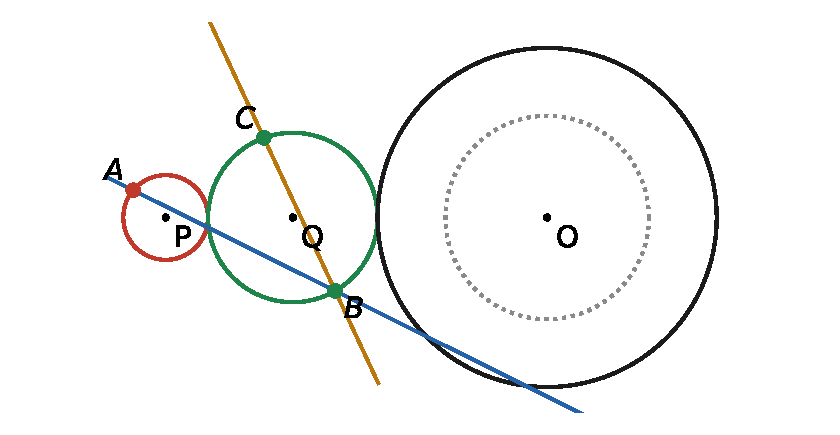
\includegraphics[width=0.72\textwidth]{fig_config.pdf}
\caption{Radii $\tfrac12$, $1$, $2$. Here the line $AB$ (blue) meets the third circle and the chord line $BC$ (orange) misses it. Both events have probability about $0.51$, and the two lines also meet the dotted circle, or any other circle about $O$, equally often.}
\label{fig:config}
\end{figure}

For equal radii, Dan found by integration that both probabilities equal
\[
\tfrac34-\tfrac{2}{\pi^2}\Bigl(\tfrac38\ln^2 2+\operatorname{Li}_2(-\sqrt2)+3\operatorname{Li}_2(\tfrac{1}{\sqrt2})\Bigr)\approx 0.3871,
\]
and asked on Mathematics Stack Exchange why they agree~\cite{MSE}. Lim Jeck gave a geometric proof and chronondecay showed more: the distances from $O$ to the two lines have the same distribution~\cite{MSE}. Dan then noticed numerically that the equality persists whenever $ac=b^2$, and asked on MathOverflow for a reason~\cite{MO}. Tom Sirgedas commented that it seems to persist when the third circle is replaced by any circle about $O$~\cite{MO}.

\emph{Before reading on, try the simplest version.} Replace the third circle by its centre and move that centre to $Q$. Is the distance from $Q$ to $AB$ distributed like the distance from $Q$ to $BC$? For $BC$ the answer is a short exercise with inscribed angles. For $AB$ the line is pulled towards the other circle, and it is not at all plain that nothing changes. Section~\ref{sec:lemma} shows that nothing does, and the rest of the paper follows from that.

\emph{Results.} Lemma~\ref{lem:two} is the two-circle fact. Theorem~\ref{thm:char} decides, for every point $O$ on the line of centres, whether the two distances agree in law. Corollary~\ref{cor:dan} answers Dan's and Tom Sirgedas's questions for every ratio, Corollary~\ref{cor:chain} extends them along chains of circles, and Corollary~\ref{cor:constant} writes Dan's constant as $\frac{2}{\pi^2}\int_0^{\pi/2}\arccos(2\cos v-1)\,dv$. Corollary~\ref{cor:ratio} gives the corresponding integral for every ratio and shows that the probability increases from $0$ to $1$ as the last circle grows.

\emph{Notation.} Put $P$ and $Q$ on the horizontal axis with $P$ to the left, and write $D=|PQ|$. Except for vertical lines, which occur with probability zero, every line has a unit normal $m=(\cos\varphi,\sin\varphi)$ with $0<\varphi<\pi$, and an equation $m\cdot z=p$. The signed distance of a point $X$ from the line is $p-m\cdot X$. The \emph{arcsine law} is the law of $\cos U$ with $U$ uniform on $[0,2\pi)$; it has density $1/(\pi\sqrt{1-x^2})$ on $(-1,1)$. Throughout, $U$ and $V$ are independent and uniform on $[0,2\pi)$.

\section{One circle}\label{sec:one}

Take the chord line $BC$ of the circle of radius $b$ about $Q$. Its signed distance from $Q$, in units of the radius, is
\[
x_B=\frac{p-m\cdot Q}{b}=\frac{m\cdot(B-Q)}{b}=\cos\theta_B,
\]
where $\theta_B$ is the angle between the radius $QB$ and the normal $m$. For example, if $BC$ is a diameter then $\theta_B=\pi/2$ and $x_B=0$; if $C$ is close to $B$ the line is nearly tangent and $x_B$ is close to $\pm1$.

\begin{lemma}\label{lem:one}
For the line $BC$, the normal angle $\varphi$ is uniform on $(0,\pi)$, the offset $x_B$ has the arcsine law, and the two are independent.
\end{lemma}

\begin{proof}
Fix $B$. As $C$ makes one full turn at constant speed, the inscribed-angle theorem makes the chord direction make a half-turn at constant speed. Thus $\varphi$ is uniform on $(0,\pi)$ whatever $B$ is. Hence $\varphi$ is independent of $B$. Writing $B-Q=b(\cos\beta,\sin\beta)$ with $\beta$ uniform, $x_B=\cos(\beta-\varphi)$, which given $\varphi$ is the cosine of a uniform angle.
\end{proof}

\section{Two circles}\label{sec:lemma}

Now take $A$ on the circle of radius $a$ about $P$ and $B$ on the circle of radius $b$ about $Q$, and let $m$ be the normal of $AB$ chosen as in the notation. Define $x_A=m\cdot(A-P)/a=\cos\theta_A$ and $x_B=m\cdot(B-Q)/b=\cos\theta_B$ as before: the offsets of the line from the two centres, in units of the radii. Figure~\ref{fig:chords} shows them as dashed perpendiculars.

\begin{lemma}\label{lem:two}
If the two discs have disjoint interiors, then $x_A$ and $x_B$ are independent and each has the arcsine law. Equivalently, the angles $\theta_A$ and $\theta_B$ are independent and uniform on $[0,\pi]$.
\end{lemma}

The convention on $m$ matters. If we instead turned $m$ so that $x_B\ge0$, the law of $x_B$ would fold in half. The hypothesis matters too: Section~\ref{sec:remarks} shows that the lemma fails for overlapping discs.

\begin{figure}[ht]
\centering
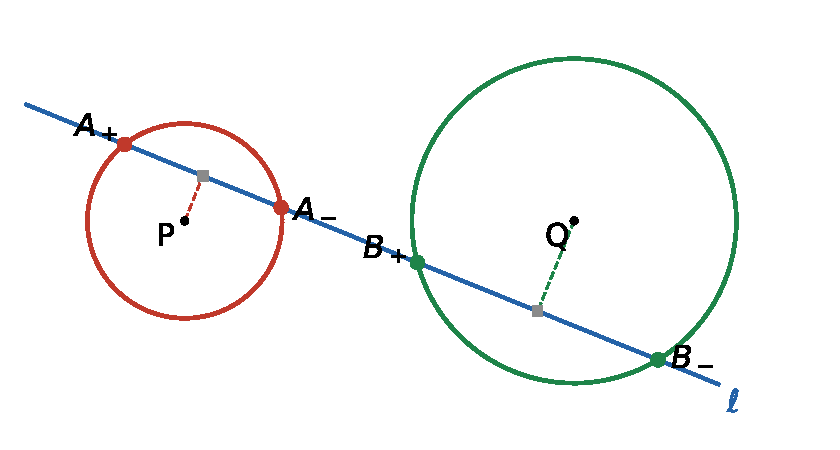
\includegraphics[width=0.74\textwidth]{fig_chords.pdf}
\caption{A line $\ell$ through both circles, at signed distance $a x_A$ from $P$ and $b x_B$ from $Q$ (dashed). It carries four pairs $(A_\pm,B_\pm)$. Each gap from an $A_\pm$ to a $B_\pm$ is the gap $g$ between the feet of the perpendiculars, plus or minus two half-chords, and the half-chords cancel when the four gaps are added.}
\label{fig:chords}
\end{figure}

\emph{The idea.} Fix the two angles $\theta_A,\theta_B$ between the normal and the radii. Their cosines are the two offsets, so they fix the line. Each radius can lie on either side of its perpendicular foot, giving four pairs $(A,B)$ on that line. The pairs are not equally likely, but their contributions add to a constant: the two half-chords cancel. For example, take unit circles with $D=3$ and offsets $x_A=0.6$, $x_B=0$. The half-chords are $0.8$ and $1$, and the feet are $g=3\sqrt{0.96}\approx2.94$ apart. The four gaps are $g\pm1.8$ and $g\pm0.2$, whose sum is $4g$.

\begin{proof}
Put $P=(-D,0)$ and $Q=(0,0)$, with $D\ge a+b$. Let $\alpha,\beta$ be the independent uniform polar angles of $A,B$. We compute their change of variables in the reverse direction: from $\theta_A,\theta_B$ to $\alpha,\beta$.

\emph{The four pairs.} The offset equations give
\[
D\cos\varphi=a\cos\theta_A-b\cos\theta_B.
\]
For $0<\theta_A,\theta_B<\pi$ this determines a unique $0<\varphi<\pi$. The four pairs have polar angles
\[
\alpha=\varphi+\varepsilon\theta_A,\qquad
\beta=\varphi+\eta\theta_B \pmod{2\pi},\qquad \varepsilon,\eta\in\{-1,1\}.
\]
Write $g=D\sin\varphi$ for the gap between the perpendicular feet, and $u=a\sin\theta_A$, $v=b\sin\theta_B$ for the half-chords. The four point-to-point gaps are $g+\varepsilon u-\eta v$. They are nonnegative because the two chords have disjoint interiors.

\emph{The density.} Differentiating the equation for $\varphi$ gives
\[
\frac{\partial\varphi}{\partial\theta_A}=\frac{u}{g},\qquad
\frac{\partial\varphi}{\partial\theta_B}=-\frac{v}{g}.
\]
For each of the four pairs, the change-of-variables determinant is therefore
\[
\left|\frac{\partial(\alpha,\beta)}{\partial(\theta_A,\theta_B)}\right|
=\left|\det\begin{pmatrix}
\varepsilon+u/g&-v/g\\ u/g&\eta-v/g
\end{pmatrix}\right|
=1+\varepsilon\frac{u}{g}-\eta\frac{v}{g}.
\]
In words, each pair contributes its gap divided by the feet-to-feet gap. Since the density of $(\alpha,\beta)$ is $1/(4\pi^2)$, summing these four contributions cancels the half-chords and gives
\[
f_{\theta_A,\theta_B}=\frac{1}{4\pi^2}
\sum_{\varepsilon,\eta}\left(1+\varepsilon\frac{u}{g}-\eta\frac{v}{g}\right)
=\frac{1}{\pi^2}.
\]
This is the density of two independent uniform angles on $(0,\pi)$. Taking their cosines gives the two independent arcsine offsets. Tangencies and coincident points in the touching case form null sets and do not affect the calculation.
\end{proof}

Each pair's contribution is an instance of a classical formula. For the line $G$ through points on two curves, $|t_2-t_1|\,dG=\sin\theta_1\sin\theta_2\,ds_1\,ds_2$, where $t_2-t_1$ is the gap between the points and $\theta_1,\theta_2$ are the angles between $G$ and the tangents~\cite[(3.30) and (4.2)]{Santalo}. For our circles these angles are $\theta_A,\theta_B$, the arc elements are $a\,d\alpha$ and $b\,d\beta$, and $dG=(uv/g)\,d\theta_A\,d\theta_B$, so the formula gives the determinant above. What is special to circles is that the four contributions add to a constant.

The lemma also gives the direction of $AB$: the cosine of its \emph{normal's} angle with the line of centres has the law of $(a\cos U-b\cos V)/D$. The line itself is perpendicular to that normal.

\section{Which centres see the two lines alike}\label{sec:char}

Let $O$ lie on the line of centres. Write $O-Q=-\mu(P-Q)$, so $\mu\ge0$ puts $O$ beyond $Q$, away from $P$, at distance $|QO|=|\mu| D$. Write $T_{AB}$ and $T_{BC}$ for the signed distances from $O$ to the two lines.

\emph{An example first.} Take Figure~\ref{fig:config}: $a=\tfrac12$, $b=1$, $D=\tfrac32$, $|QO|=3$, so $\mu=2$. Project everything onto the normal $m$ of $AB$ (Figure~\ref{fig:proj}). The line becomes the single number $p$, the centres become the numbers $m\cdot P$, $m\cdot Q$, $m\cdot O$, and projection keeps the ratio $\mu$: $m\cdot O-m\cdot Q=-2\,(m\cdot P-m\cdot Q)$. The line sits at $a x_A=\tfrac12x_A$ from $m\cdot P$ and at $x_B$ from $m\cdot Q$, so $m\cdot P-m\cdot Q=x_B-\tfrac12x_A$, and
\[
T_{AB}=p-m\cdot O=x_B+2\bigl(x_B-\tfrac12x_A\bigr)=3x_B-x_A.
\]
By Lemma~\ref{lem:two} this is a sum of independent arcsine variables with weights $3$ and $1$. For the chord, Lemma~\ref{lem:one} gives $T_{BC}=x_B-3\cos\varphi$, again weights $1$ and $3$. The same weights in a different order, so the same law.

\begin{figure}[ht]
\centering
\begin{tikzpicture}[x=2.2cm,y=1cm,>=stealth]
\draw[->] (-0.4,0) -- (3.4,0) node[right] {$m\cdot z$};
\foreach \x/\l in {0/{m\cdot P},1/{m\cdot Q},3/{m\cdot O}} {\fill (\x,0) circle (1.6pt); \node[below] at (\x,-0.05) {$\l$};}
\draw[very thick,blue] (1.6,-0.25) -- (1.6,0.25); \node[blue,below] at (1.6,-0.3) {$p$};
\draw[<->] (0,0.55) -- node[above] {$a x_A$} (1.6,0.55);
\draw[<->] (1,1.15) -- node[above] {$b x_B$} (1.6,1.15);
\draw[<->] (3,0.55) -- node[above] {$T_{AB}$} (1.6,0.55);
\draw[dashed,gray] (0,0) -- (0,0.7) (1,0) -- (1,1.3) (1.6,0.25) -- (1.6,1.3) (3,0) -- (3,0.7);
\end{tikzpicture}
\caption{Projection onto the normal of $AB$. The line becomes the point $p$, the three centres keep their ratio $\mu$ (here $2$), and the offset $T_{AB}$ of $p$ from $m\cdot O$ is read off by extrapolating from the two known offsets.}
\label{fig:proj}
\end{figure}

The same projection works for every $O$ on the line of centres:
\begin{equation}\label{eq:T}
T_{AB}=(1+\mu)\,b\,x_B-\mu\,a\,x_A,\qquad T_{BC}=b\,x_B-\mu D\cos\varphi .
\end{equation}
In words, the line's offset from $O$ is its offset from $Q$, extrapolated along the projected axis by the change in offset between $P$ and $Q$. So both distances are weighted sums of two independent arcsine variables. All that remains is to know when two such sums agree in distribution. For weights $3$ and $1$, the largest possible absolute value is $4$ and the mean squared value is $(3^2+1^2)/2=5$. These two quantities already determine the two weights.

\begin{lemma}\label{lem:moments}
Let $\alpha,\beta,\gamma,\delta$ be real. Then $|\alpha\cos U+\beta\cos V|$ and $|\gamma\cos U+\delta\cos V|$ have the same law if and only if $\{|\alpha|,|\beta|\}=\{|\gamma|,|\delta|\}$.
\end{lemma}

\begin{proof}
Signs do not matter because $\cos U$ and $-\cos U$ have the same distribution, and the two weights may be swapped. Conversely, the distribution of $|X|$, where $X=\alpha\cos U+\beta\cos V$, determines
\[
M=|\alpha|+|\beta|,\qquad
2\E|X|^2=\alpha^2+\beta^2.
\]
Here $M$ is the upper endpoint of its support: values arbitrarily close to it occur with positive probability. These two quantities give $|\alpha\beta|=(M^2-2\E|X|^2)/2$, so $|\alpha|,|\beta|$ are the two roots of $t^2-Mt+|\alpha\beta|=0$.
\end{proof}

\begin{theorem}\label{thm:char}
Let two circles, of radii $a$ and $b$ about $P$ and $Q$, bound discs with disjoint interiors. Let $A$ be uniform on the first circle and $B$, $C$ uniform on the second, all independent, and let $O$ be a point on the line $PQ$. Then $d(O,AB)$ and $d(O,BC)$ have the same law if and only if
\begin{enumerate}
\item $O=Q$, or
\item the circles touch, and $O$ lies on the ray from $Q$ away from $P$ with $|QO|=b(a+b)/a$.
\end{enumerate}
In either case the common law is that of $|\,b\cos U-|QO|\cos V\,|$.
\end{theorem}

\begin{proof}
By~\eqref{eq:T} and Lemmas~\ref{lem:one} and~\ref{lem:two}, $d(O,AB)$ and $d(O,BC)$ are the absolute values of weighted sums of two independent arcsine variables, with weights $\{|1+\mu|\,b,\;|\mu|\,a\}$ and $\{b,\;|\mu|D\}$. By Lemma~\ref{lem:moments} the laws agree exactly when these unordered pairs agree. There are two ways to match them.

If $|1+\mu|b=b$ and $|\mu|a=|\mu|D$, then $\mu\in\{0,-2\}$, and $\mu=-2$ would force $a=D$, which is impossible since $D\ge a+b$. So $\mu=0$, which is case (1).

If $|\mu|a=b$ and $|1+\mu|b=|\mu|D$, then $|\mu|=b/a$ and
\[
|1+\mu|=\frac{D}{a}\ \ge\ \frac{a+b}{a}=1+|\mu|.
\]
The triangle inequality gives $|1+\mu|\le1+|\mu|$, so both inequalities are equalities: $D=a+b$, so the circles touch, and $\mu=b/a\ge0$. Then $|QO|=\mu D=b(a+b)/a$, which is case (2). Each step reverses, so both cases do give equal laws.
\end{proof}

In case (2), the circle about $O$ that touches the second circle has radius $c=|QO|-b=b^2/a$. That is Dan's condition $ac=b^2$.

\section{Consequences}\label{sec:cons}

\begin{corollary}\label{cor:dan}
For three touching circles with collinear centres and $ac=b^2$, the distances from $O$ to $AB$ and to $BC$ have the law of $|b\cos U-(b+c)\cos V|$. So, for every $\rho>0$, the two lines meet the circle of radius $\rho$ about $O$ with the same probability. If $ac\ne b^2$, the two distance laws differ.
\end{corollary}

\begin{proof}
Apply Theorem~\ref{thm:char} with $|QO|=b+c$. A line meets the circle of radius $\rho$ about $O$ exactly when its distance from $O$ is at most $\rho$.
\end{proof}

Taking $\rho=c$ answers Dan's question for every ratio, and the free radius $\rho$ is Tom Sirgedas's observation. The converse concerns equality for every radius: different distance laws need not give different hit probabilities at any particular radius.

The theorem is symmetric under swapping the two circles: the line $AB$ and a chord $AA'$ of the first circle are at the same distance in law from the point beyond $P$ at distance $a(a+b)/b$, the centre of the next circle in the progression on that side. Applying both versions along a row gives the following.

\begin{corollary}\label{cor:chain}
Let circles $\Gamma_k$ with radii $r^k$ ($k\in\mathbb{Z}$) touch in a row with collinear centres $O_k$, and choose independent uniform points $A_k,A'_k$ on each $\Gamma_k$. Then $d(O_{k+2},A_kA_{k+1})\eqd d(O_{k+2},A_{k+1}A'_{k+1})$ and $d(O_{k-1},A_kA_{k+1})\eqd d(O_{k-1},A_kA'_k)$ for every $k$.
\end{corollary}

How does the common hit probability change with the ratio? In Figure~\ref{fig:config}, $c/b=2$ gives about $0.51$, whereas equal radii give about $0.3871$. Scale $b$ to $1$ and put $r=c/b$. The two random lines then share the probability
\[
H(r)=\Pr\{|\cos U-(1+r)\cos V|<r\}.
\]
Increasing $r$ moves the third centre as well as enlarging its circle, but the circles remain tangent to the second circle at the same point and their discs are nested (Figure~\ref{fig:nested}).


\begin{figure}[ht]
\centering
\begin{tikzpicture}[scale=0.85]
\draw[gray!65] (0,0) circle (1);
\fill (0,0) circle (1.6pt) node[left] {$Q$};
\draw[blue!65,thick] (3,0) circle (2);
\draw[blue!80,thick] (2,0) circle (1);
\draw[blue!95,thick] (1.5,0) circle (0.5);
\fill (1,0) circle (1.6pt);
\foreach \x/\r in {1.5/{\tfrac12},2/{1},3/{2}}
{\fill (\x,0) circle (1.4pt);}
\draw[dashed,gray] (1,0) -- (5,0);

\end{tikzpicture}
\caption{Keep the second circle (grey, radius $1$) fixed. The three blue discs, from smallest to largest, have radii $r=\tfrac12,1,2$. They are nested and tangent at the same point; their centres are $1+r$ from $Q$.}
\label{fig:nested}
\end{figure}

\begin{samepage}
\begin{corollary}\label{cor:ratio}
Write $[t]_{-1}^{1}=\max(-1,\min(1,t))$ to restrict a threshold to the cosine's range. For every $r>0$,
\[
H(r)=\frac{2}{\pi^2}\int_0^{\pi/2}
\left\{\arccos\bigl([(1+r)\cos v-r]_{-1}^{1}\bigr)
-\arccos\bigl([(1+r)\cos v+r]_{-1}^{1}\bigr)\right\}\,dv.
\]
The function $H$ is continuous and strictly increasing, with $H(r)\to0$ as $r\downarrow0$ and $H(r)\to1$ as $r\to\infty$.
\end{corollary}
\end{samepage}

\begin{proof}
Given $Y=\cos V=y$, the event asks that $X=\cos U$ lie between $(1+r)y-r$ and $(1+r)y+r$. Its probability is the difference of the two arccosines divided by $\pi$, with thresholds outside $[-1,1]$ restricted to the endpoints. Reflection replaces $y$ by $-y$, so averaging over $0<v<\pi/2$ gives the formula.

The same interval can be written
\[
y-r(1-y)<X<y+r(1+y).
\]
For $-1<y<1$ it expands as $r$ grows. Every increase in $r$ adds an open region inside $(-1,1)^2$, where the joint density of $X,Y$ is positive, so $H$ increases strictly. Continuity and the two limits follow by dominated convergence: boundaries have probability zero, the interval shrinks to $\{y\}$ as $r\downarrow0$, and eventually contains $[-1,1]$ as $r\to\infty$.
\end{proof}

The equal-radius case gives Dan's constant a simpler form.

\begin{corollary}\label{cor:constant}
For $a=b=c$ and $\rho=c$, the common probability is
\[
\Pr\{|\cos U-2\cos V|<1\}=\frac{2}{\pi^2}\int_0^{\pi/2}\arccos(2\cos v-1)\,dv=0.38712871059988957\ldots
\]
\end{corollary}

\begin{proof}
Set $r=1$ in Corollary~\ref{cor:ratio}. On $0\le v\le\pi/2$, the upper threshold $2\cos v+1$ is at least $1$, while the lower threshold $2\cos v-1$ lies in $[-1,1]$. Thus the second arccosine vanishes and the first needs no restriction.
\end{proof}

The integral agrees with Dan's dilogarithm expression to 40 digits. We have not derived that expression from it.

\section{Remarks}\label{sec:remarks}

\emph{Disjointness is needed.} For overlapping discs, the chords can interleave and the four gaps no longer have one sign. A direct counterexample is provided by concentric circles: their signed offsets satisfy $a x_A=b x_B$, so they cannot be independent nonconstant random variables.

\emph{Off the axis: an exact test.} Keep $P=(-D,0)$ and $Q=(0,0)$ and write $O=(h,k)$. For example, moving the successful centre of Figure~\ref{fig:config} from $(3,0)$ to $(3,0.3)$ makes the mean squared distance to $AB$ exceed that to $BC$ by exactly $0.02$. No simulation is needed to separate the distributions.

To obtain the test, put $X=x_A$, $Y=x_B$ for $AB$. Lemma~\ref{lem:two} and $D\cos\varphi=aX-bY$ give
\[
T_{AB}=bY-\frac{h}{D}(aX-bY)
-k\sqrt{1-\frac{(aX-bY)^2}{D^2}}.
\]
The first two terms are the axial extrapolation; the last is the perpendicular displacement projected onto the normal. Under $(X,Y)\mapsto(-X,-Y)$, the axial part changes sign and the square root does not, so their cross term has expectation zero. Using $\E X^2=\E Y^2=1/2$ and $\E XY=0$, and $\E d(O,BC)^2=(b^2+h^2+k^2)/2$ from Lemma~\ref{lem:one}, gives
\begin{equation}\label{eq:offaxis}
\E d(O,AB)^2-\E d(O,BC)^2
=\frac{\Delta(k^2-h^2)+2b^2Dh}{2D^2},
\qquad \Delta=D^2-a^2-b^2>0.
\end{equation}
Thus equality of the distance distributions requires
\[
h^2-k^2=\frac{2b^2D}{\Delta}\,h.
\]
In particular, any nonzero perpendicular displacement from either centre identified in Theorem~\ref{thm:char} destroys equality: it increases the difference of the mean squared distances by $\Delta k^2/(2D^2)>0$. Other points on this hyperbola remain candidates; the test alone does not characterise off-axis equality.

\emph{Related results.} Lim Jeck's argument~\cite{MSE} for $a=b=c$ compares tangent lines with the projection law of the circle; the author's MathOverflow answer~\cite{MOA} extends it to equal hit probabilities whenever $ac=b^2$. chronondecay~\cite{MSE} proved the distributional statement for $a=b=c$ by a different geometric route. In three dimensions, the line through two independent uniform points of $S^2$ is distributed according to the Crofton measure~\cite[Lemma~8]{AEN}, so its entry and exit points are independent, and Bilyk, Chang, Hein\"avaara, Matzke and Steinerberger~\cite{BCHMS} show that among smooth convex bodies only the ball in $\R^3$ has this property. Lemma~\ref{lem:two} is a planar statement of the same kind for two circles. Its change of variables is classical, as noted after its proof, but we have not found the four-gap cancellation or the lemma itself stated.

\emph{Verification.} Scripts check the change-of-variables calculation, the weight comparison and centre classification, the off-axis second-moment identity, and the hit-probability integrals. They include exact rational checks, numerical illustrations and deliberately false variants that must fail. The proofs do not depend on these scripts, which serve as a guard against slips in the algebra. They are at
\begin{center}\small\url{https://github.com/jvvk/mathematics/tree/main/random-chords-two-circles}.\end{center}

\section*{Acknowledgements}

The question and its numerical evidence are Dan's; the observation about other radii is Tom Sirgedas's; the equal-radius proofs are Lim Jeck's and chronondecay's. Claude Opus 5.5 (Anthropic) found Lemma~\ref{lem:two}, Theorem~\ref{thm:char} and their proofs, ran the numerical checks and drafted this paper, and OpenAI Codex extended Lim Jeck's argument to $ac=b^2$, simplified the change-of-variables and weight-comparison proofs, and added Corollary~\ref{cor:ratio} and the off-axis second-moment test. The author has checked the arguments and is responsible for the content.

\begin{thebibliography}{9}
\bibitem{AEN} A.~Akopyan, H.~Edelsbrunner and A.~Nikitenko, \emph{The beauty of random polytopes inscribed in the $2$-sphere}, Experiment.\ Math.\ \textbf{34} (2025), no.~3, 327--341. \href{https://doi.org/10.1080/10586458.2021.1980459}{doi:10.1080/10586458.2021.1980459}.
\bibitem{BCHMS} D.~Bilyk, A.~Chang, O.~Hein\"avaara, R.~W.~Matzke and S.~Steinerberger, \emph{A random line intersects $\mathbb{S}^2$ in two probabilistically independent locations}, J.\ Geom.\ Anal.\ \textbf{35} (2025), article 263. \href{https://doi.org/10.1007/s12220-025-02094-1}{doi:10.1007/s12220-025-02094-1}.
\bibitem{MO} Dan, \emph{Why do these two lines have the same probability of intersecting the circle?}, MathOverflow question 499477 (22 August 2025), with comments, \url{https://mathoverflow.net/q/499477}.
\bibitem{MOA} V.~Jandhyala, answer to MathOverflow question 499477 (4 October 2026), \url{https://mathoverflow.net/a/515721}.
\bibitem{MSE} Dan, \emph{Why do these two lines have the same probability of intersecting the circle?}, Mathematics Stack Exchange question 5089940 (14 August 2025), with answers by Lim Jeck and chronondecay (29 August 2025), \url{https://math.stackexchange.com/q/5089940}.
\bibitem{Santalo} L.~A. Santal\'o, \emph{Integral Geometry and Geometric Probability}, Encyclopedia of Mathematics and its Applications~1, Addison-Wesley, Reading, MA, 1976.
\end{thebibliography}

\end{document}
